\chapter{Networks}
\label{chap:networks}
\section{Introduction}
The structure of a network can be descibed by a $n \times n$ matrix: the (weighted) adjacency matrix $A = \{\mathbf{A}_{ij}\}$. If two nodes $i$ and $j$ are not joined by a link, $A_{ij} = 0$. Otherwise, $A_{ij} = 1$ (for binary networks) or $A_{ij} \in \mathbb{R} - \{0\}$ (for weighted networks). For binary directed networks $A_{ij} = 1$ if there is an edge from $i$ to $j$. For undirected networks the adjacency matrix is symmetric, $\mathbf{A} = \mathbf{A}^T$. Usually, $A_{ii} = 0$ for any $i$ (no self-edges).
\begin{mydefinition}[Walk, trail, path, length]
 \begin{itemize}
 	\item A walk is any sequence of edges which joins a sequence of vertices
 	\item A trail is a walk in which all edges are distinct
 	\item A path is a trail in which all vertices (and therefore also all edges) are distinct
 	\item The length of a walk/trial/path is the number of edges traversed along the path
 \end{itemize}
\end{mydefinition}
The total number of path of length 2 from $i$ to $j$ is:
\[
N_{ij}^{(2)} = \sum_{k=1}^{n} A_{ik}A_{kj} = (A^2)_{ij}
\]
and in general the number of walks connecting $i \to j$ of length $r$ is $(A^r)_{ij}$
\newpage
\begin{mydefinition}[Cycles]
A cycle is any walk/trial/path $i \to i$ (initial node and final one are the same). The total numer of cycles of length $r$ is:
\[
L_r = \sum_{i =1}^{n} (A^r)_{ii} = \text{Tr}[A^r]
\]
\end{mydefinition}
For symmetric networks, the adjacency matrix is symmetric, eigenvalues are real and it can be diagonalized as:
\[
\mathbf{A} = \mathbf{U}\mathbf{\Lambda} \mathbf{U}^T
\]
where $\Lambda$ is the diagonal matrix of eigenvalues $\lambda_i$ and $U$ is the orthogonal matrix of eigenvectors (arranged in columns). Then $A^r = (U\Lambda U^T)^r = U\Lambda^rU^T$ and:
\[
L_r = \text{Tr}[\mathbf{U}\mathbf{\Lambda}^r\mathbf{U}^T] = \text{Tr}[\mathbf{\Lambda}^r] = \sum_{i=1}^n \lambda_i^r 
\]
That relation is true from any networks (proof using Schur decomposition)
\begin{mydefinition}[Acyclic Directed Networks or Directed Acyclic Graph (DAG)]
A cycle in a directed network is a closed loop of edges with the arrows on each edge pointing in the same direction around the loop. Directed networks without cycles are acyclic. One can always depict a DAG in a ordered way - vertices running from top to bottom, all edges point downward.
\end{mydefinition}
 By using the sorting of nodes in the previous representation, the adjacency matrix becomes (strictly) upper triangular.
 \begin{mytheorem} [Eigenvalues acyclic network]
 The eigenvalues of the adjacency matrix are all zero if and only if the network is acyclic, then the total number $L_r$ of cycles of length $r$ is:
 	\[
 	L_r = \sum_{i =1}^n \lambda_i^r
 	\]
 \end{mytheorem}
\begin{mydefinition}
A tree is a connected, undirected network that contains no closed loops. (Connected means that every vertex is reachable from every other via some path).\\
A network consisting of more than one componenet, each being a tree, is a forest.
\end{mydefinition}
\begin{mytheorem}[Condition for existence of tree]
	A network is a tree if and only if it is connected and has $n-1$ edges.
\end{mytheorem}
\begin{mydefinition}
A planar network is a network that can be drawn on a plane without having any edges cross. Two important examples of non-planar networks
\end{mydefinition}
$K_5$ is the complete graph with 5 vertices. UG is the complete bipartite graph on two groups of three vertices.
\begin{mytheorem}[Kuratowski's theorem]
	Every non-planar networks contains at least one subgraph that is an expansion of $K_5$ or UG
\end{mytheorem}
\begin{center}
	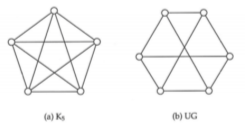
\includegraphics[width=0.5\textwidth]{picture/(40)k5_ug.png}
\end{center}
The (binary) network is represented by the $n\times m$ incidence matrix $B$ (the equivalent of the adjacency matrix).One-mode projection is a unipartite network where nodes are linked if they share at least one node of the second type. Nodes of type $A$ connected to the same node of type $B$ form a clique in the projected network. 
\begin{mydefinition}[Weighed adjacency Matrix Bipartite network]
In bipartite network:
\[
A_{ij} = \sum_{k=1}^{m}B_{ki} B_{kj} = \sum_{k=1}^{m} B_{ik}^TB_{kj} 
\]
\end{mydefinition}
However the diagonal elements are $A_{ij} = \sum_{k=1}^m B_{ki}^2 \neq 0$ and should be set to zero by hand.
The ptjer projecton gives $P = BB^T$
\newpage
\section{Graph Laplacian}
\begin{mydefinition}[Graph Laplacian]
	The graph Laplacian is the matrix is $\mathbf{L} = \mathbf{D} - \mathbf{A}$
\end{mydefinition}
We can write a diffusion equation as:
\[
\frac{d \vec{\psi}}{dt} + cL \vec{\psi} = 0
\]
similar to $\partial_t \vec{\psi} + c \lambda^2 \vec{\psi} = 0$.\\
The solution of the diffusion equation can be found by setting:
\[
\vec{\psi}(t) = \sum_i a_i(t) \vec{v}_i
\]
where $\vec{v}_i$ are the eigenvectors of $L$ assocaited to the eigenvalues $\lambda_i$. Substituting we get:
\[
\dot{a}_i + c\lambda_i a_i = 0
\]
with solution:
\[
a_i(t) = a_i(0)e^{-c\lambda_it}
\]
The diffusion is governed by $\{\lambda_i\}$.\\
Let us analyse the eigenvalues of graph Laplacian:
\begin{itemize}
\item $\lambda_i \in \mathbb{R}$ for any $i$ ($\mathbf{L}$ is symmetric if network is undirected) and $\lambda_i \geq 0 \quad \forall i$ (it can be proof through an edge incidence matrix $\mathbf{B}$). From this we see that diffusion over a network is never an exploding process.
\item At least one eigenvalue is zero. This can be seen as a conservative law.
\item If the network is divided in $k$ disconnected components, the adjency matrix and the Laplacian are block diagonal: in similar way of above, for each block leads to other $k$ eigenvalues equal to zero (never exist a link between a group and another one)
\item The second largest eigenvalue of the graph Laplacian is non-zero $\iff$ the network is connected. This eigenvalue is called algebraic connectivity or spectral gap of the network.
\end{itemize}
\section{Random walk on a network}
A random walk on a network is a walk defined by a sequence of random steps, it is useful finding the probability $p_i(t)$ that the walker is at node $i$ at time $t$.\\
The possible steps from generic $j$, it is the uniform probability $1/k_j$ of taking a step along one of the $k_j$ edges incident to $j$ times the probability to be in $j$ at time $t-1$. Summer over all possible $j$ we find a recursive formula:
\[
p_i(t) = \sum_j \frac{A_{ij}}{k_j} p_j(t-1)
\] 
In the limit $t\to \infty$ the stationary probability is:
\[
\vec{p} = \mathbf{A}\mathbf{D}^{-1}\vec{p} \to (\mathbf{I} - \mathbf{A}\mathbf{D}^{-1})\vec{p} = (\mathbf{D}-\mathbf{A})\mathbf{D}^{-1}\vec{p} = \mathbf{L}\mathbf{D}^{-1}\vec{p}=0
\]
In case network is connected $\mathbf{D}^{-1}\vec{p} =a\vec{1} \to \vec{p} = a\mathbf{D}\vec{1} \to p_i = ak_i$, then:
\[
p_i = \frac{k_i}{\sum_i k_i} = \frac{k_i}{2m}
\]
The probability of a random walk is proportional to the degree.
\subsection{Mean first passage time}
The first passage time for a random walk from a vertex $u$ to a vertex $v$ is the number of steps before a walk starting at $u$ reaches $v$. First passage time is a random variable, we want to find the mean value.\\
To evaluate it, we model an absorbing random walk: if the walk reaches $v$ it remains there forever.\\
Let $p_v(t)$ be the probability that the walker is at $v$  (absorbed) at time $t$.\\
$p_v(t)$ is also the probability that the walk has a first passage time to $v$ that is less than or equal to $t$. For this, the probability that the walk has a first passage time to $v$ exactly at time $t$ is $p_v(t) - p_v(t-1)$. Until now, we can express the mean first passage time as:
\[
\tau_v = \expected{t} = \sum_{t =0}^{\infty} t[p_v(t) - p_v (t-1)]
\]
$\forall i \neq v$:
\[
p_i(t) = \sum_j \frac{A_{ji}}{k_j}p_j(t-1) = \sum_{j \neq v} \frac{A_{ij}}{k_j} p_j (t-1)
\]
because $a_{iv} = 0$ (absorbing state). If $i\neq b$, there are no terms in $A_{vj}$ in the sum either thus we can write:
\[
\vec{p}'(t) = \mathbf{A}'\mathbf{D}'^{-1}\vec{p}'(t-1) = [\mathbf{A}'\mathbf{D}'^{-1}]\vec{p}'(0)
\]
where we have used:
\[
\sum_{t=0}^{\infty} t [ \mathbf{M}^{t-1} - \mathbf{M}^t] = [\mathbf{I} - \mathbf{M}]^{-1}
\]
We transformed a stochastic problem in a deterministic one.\\
Since
\[
[\mathbf{I} - \mathbf{A}'\mathbf{D}'^{-1}]^{-1} = \mathbf{D}'[\mathbf{D}'- \mathbf{A}']^{-1} = \mathbf{D}'\mathbf{L}'^{-1}
\]
obtaining:
\[
\tau_v = \vec{1}^T \mathbf{D}'\mathbf{L}'^{-1}\vec{p}'(0)
\]
$\mathbf{L}'$ is the graph Laplacian where the $v-th$ row and column are removed and is called reduced Laplacian.\\
\section{Random Graph}
A random graphs define a probability space or networks ensemble $(\Theta, \mathcal{A}, \mathbb{P})$, with:
\begin{itemize}
	\item $\Theta$ the sample space for graphs: $\Theta \in \{0,1\}^{n \times n}$
	\item $\mathcal{A}$ the $\sigma-$algebra on $\Theta$
	\item $\mathbb{P}: \mathcal{A} \to [0,1]$ some properly defined probability measure
\end{itemize}
\subsection{Erd\"{o}s-Rèny}
That is a random graph defines by two variables $G(n.m)$, $m$ is the average number of edges.\\
The average node degree is $\expected{k} = 2m/n$. However it is difficult to work with $G(n,m)$ becaus it is difficult, first of all counting the $\Gamma$ graphs with ecactly $n$ nodes and $m$ edges.\\
It is better working with $G(n,p)$ where each edge is Bernoulli random variable with probability $p$.\\
In this graph:
\[
\mathbb{P}(G) = p^m (1-p)^{{n \choose 2} -m}
\]
The mean value of $m$ is:
\[
\expected{m} = \sum_{m=0}^{\infty} m\mathbb{P}(m) = {n \choose 2} p
\]
The mean degree is:
\[
\expected{k} = \sum_{m =0}^{\infty} \frac{2m}{n} \mathbb{P}(m) = \ldots = (n-1)p
\]
we define the mean degree with $c$.\\
It is possible show that degree distribution is a Poisson distribution:
\[
p_k \sim e^{-c} \frac{c^k}{k!}
\]
In this graph, the expected clustering coefficient is given by:
\[
\expected{C_i} =p= \frac{c}{n-1}
\]
Let us analyse the eigenvalues: plotting the eigenvalues histogram for a random graph at different $p$:
\begin{center}
	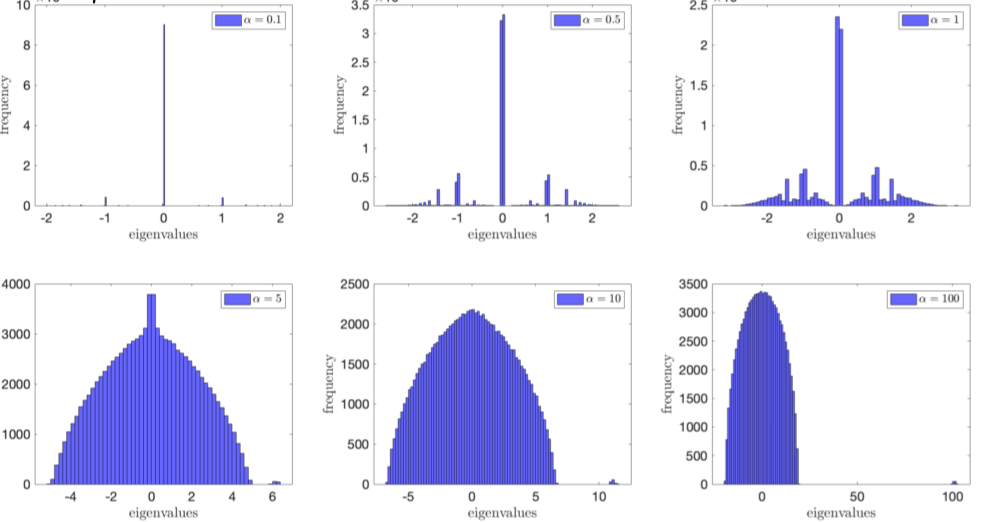
\includegraphics[width=0.5\textwidth]{picture/(42)eigenvalues_random.png}
\end{center}
\subsection{Wigner matrices}
\begin{mydefinition}[Wigner matrices]
Let $Y_n$ a $n \times n$ symmetric (or Hermitian) matrix with $\{Y_{ij}\}_{j>i,i=1,\ldots,n}$ and $\{Y_{ii}\}_{i =1,\ldots,n}$ two sets of i.i.d random variables with $\expected{Y_{ij}} = 0$ for any $i,j$. Then the matrix:
\[
X_n = n^{-1/2}Y_n
\]
with $\expected{X_{ij}} = \sigma^2 <\infty$ is a Wigner matrix
\end{mydefinition}
\begin{mytheorem}[Eigenvalues distribution Wigner matrix]
	For a Wigner matrix satisfying the Lindeberf's condition (th central limit $\to$ converge to a distribution) the sequence of eigenvalue Empricial Density Function (EDF) $F^W$ converges weakly to the Wigner semicircle law in almost sure sense, i.e. $\forall f$ bounded and continuous:
	\[
	\int f(x)F^W(x)dx \xrightarrow[]{\text{a.s.}} \int f(x) \mu_{sc} (x, \sigma^2)dx
	\]
where:
\[
\mu_{sc}(x,\sigma^2) = \frac{1}{2 \pi \sigma^2}\sqrt{4\sigma^2 -x^2}
\]
\end{mytheorem}
The semicircle law for $X_n = n^{-1/2}Y_n$ implies that the distribution of eigenvalues of $Y_n$ is scaling as:
\[
\rho(\lambda) = \frac{1}{2 \pi \sigma^2 n}\sqrt{4 n \sigma^2 - \lambda^2}
\]
\section{Random Graph eigenvalues}
In order to study the distribution of the eigenvalues, we need to normalize the adjacency matrix $\mathbf{A}$:
\[
\hat{\mathbf{A}} = (np(1-p))^{-1/2} \mathbf{A} \to \expected{\hat{A}_{ij}} = (np(1-p))^{-1/2}p, \qquad Var[\hat{A}_{ij}] = n^{-1}
\]
Than $\hat{\mathbf{A}} = \bar{\mathbf{A}} + \tilde{\mathbf{A}}$ with:
\begin{itemize}
	\item $\hat{A}_{ij} = (np(1-p))^{-1/2}p$ mean of $A_{ij}$
	\item $\tilde{A}_{ij}$ are i.i.d random variables with zero mean and variance 1/$n$.
	\item The Wigner's semicircle law hold for $\tilde{\mathbf{A}}$ and the Wigner theorem ensures that $||\tilde{\mathbf{A}}||_2 = 2$
\end{itemize}
To determine the eigenvcalues of $\mathbf{A}$ we use two lemmas:
\begin{mytheorem}[Lemma 1: Inequality Distribution]
	If $F^{X_1}(x)$ and $F^{X_2}(x)$ are eigenvalue EDF of $X_1$ and $X_2$ symmetric matrices of size $n$, then:
	\[
	|F^{X_1}(x) - F^{X_2}(x)| \leq \frac{\text{rank}(X_1-X_2)}{n}
	\]
\end{mytheorem}
So since $\hat{\mathbf{A}}$ has tank 1 for any $n$, when $n \to \infty$ the two eigenvalues EDFs vecome equal, thus the EDF of $\hat{\mathbf{A}}$ is the semicircle law.
\begin{mytheorem}[Bauer-Fike theorem]
	For symmetric matrices with $\hat{\mathbf{A}} - \hat{\mathbf{A}} = \tilde{\mathbf{A}}$, it is:
	\[
|\lambda_i(\hat{\mathbf{A}}) - \lambda(\bar{\mathbf{A}})\leq ||\tilde{\mathbf{A}}||_2 = 2
	\]
\end{mytheorem}
This theorem is usegul for the largest eigenvalue. Since $\lambda(\hat{A}) = np/\sqrt{np(1-p)} = \sqrt{np/(1-p)}$, it is:
\[
\Big| \lambda_1(\hat{\mathbf{A}}) - \sqrt{\frac{np}{1-p}}\Big|\leq 2
\]
and:
\[
\lambda_1(\hat{\mathbf{A}}) \xrightarrow[n \to \infty]{\text{a.s.}}\sqrt{\frac{np}{1-p}}
\]
Finally, remembering that $\mathbf{A} = \sqrt{n(1-p)}\hat{\mathbf{A}}$, the spectrum of the adjacency matrix $G(n,p)$ is composed by large eigenvalue:
\[
\lambda_1(A) = np
\]
and a semicircle part with support $[-2\sqrt{np(1-p)},2\sqrt{np(1-p)}]$
\section{Clustering and partition in networks}
In a random graphs we have seen $G(n,p)$ with a mean clustering coefficient $C = \frac{c}{n-1}\to 0$ for large networks $(n \to \infty)$, however real-world networks display often some modularity structure (communities). In this case adjacency matrix show a block structure.\\
Let be $n$ the number of nodes, $q$ the number of groups and let assume that each node belongs to one of the $q$ groups.\\
\subsection{Stochastic Block Models (SBMs)}
We consider labels generation: $ i \to g_i \in \{1,\ldots,q\}$ with some probability $\mathbb{P}(g_i = a) = n_a$(for example $n_a = 1/q, \forall a = 1,\ldots,q$).\\
Define an affinity matrix (link probability within and between groups):
\[
p =
\begin{pmatrix}
	p_{11} & p_{12} & p_{13}\\
	p_{21} & p_{22} & p_{23}\\
	p_{31} & p_{32} & p_{33}
\end{pmatrix}
\]
Links generation $\mathbb{P}(A_{ij} =1) = p_{g_ig_j}$.\\
Let consider $2 \times 2$ case:
\[
p =\begin{pmatrix}
	p_{11} & p_{12}\\
	p_{21} & p_{22}
\end{pmatrix}
\]
\begin{itemize}
	\item if $p_{11},p{22}>p_{12}$ the network has a modular structural
	\item if $p_{12} > p_{11},p_{22}$ the network has a bipartite structural
	\item if $p_{11}>p_{12}>p_{22}$ the network has a core-periphery 
\end{itemize}
Case direct network: if $\expected{\text{\# forward link}} \geq \expected{\text{\# backward link}}$ the network has a hierarchical structure .\\
The Bauer-Fike theorem is a useful tool in the context of a symmetric Stochastic Block Model (SBM) with $M$ equal-sized blocks. It allows us to establish that the largest $M$ eigenvalues of the SBM are determined by the affinity matrix $p$. Here's how it works: consider a symmetric SBM with $M$ equal-sized blocks.\\
The mean adjacency matrix of this SBM can be expressed as $\expected{A} = p \otimes J_k$, where: $k = n/M$ represents the number of elements per block and $J_k$ is a $k \times k$ matrix consisting of all ones.
Now, let's consider the eigenvalues of a Kronecker product ($\otimes$). The eigenvalues of the Kronecker product of two matrices are the product of the eigenvalues of the individual matrices..\\
In this case, the Kronecker product involves $p \otimes J_k$. The largest eigenvalue of this product is $z_1n/M$, where:$z_1$ is the largest eigenvalue of the affinity matrix $p$.\\
Also in this case, let consider the case with two blocks:
\[
p = \begin{pmatrix}
	p_{11} & p_{12}\\
	p_{12} & p_{22}
\end{pmatrix}
\]
and the two eigenvalues are:
\[
z_{1,2} = \frac{p_{11} + p_{22} \pm \sqrt{(p_{11} - p_{22})^2 + 4p^2_{12}}}{2}
\]
The first eigenvector has two components of the same sign and using Bauer-FIke we can conclude that the largest eigenvalue of the adjacency matrix of a SBM with two equal sized blocks is in the limit $n \to \infty$:
\[
\lambda_1 = \frac{p_{11} + p_{22} + \sqrt{(p_{11} - p_{22})^2 + 4 p_{12}^2}}{4}n
\]
